% A0 portrait poster macros derived from the 2025 winter statistics poster PPTX.
% Final Korean print PDFs should be compiled with XeLaTeX, Hangul Pretendard, and Cambria Math.

\usepackage[
  paperwidth=841mm,
  paperheight=1189mm,
  margin=0mm
]{geometry}
\usepackage{xcolor}
\usepackage{iftex}
\newif\ifWantedKotex
\IfFileExists{kotex.sty}{%
  \WantedKotextrue
}{%
  \WantedKotexfalse
  \PackageWarningNoLine{wanted-poster}{kotex.sty not found. Install texlive-lang-korean or compile in a Korean-capable XeLaTeX environment for Hangul text}%
}
\ifPDFTeX
  \usepackage[T1]{fontenc}
  \usepackage[utf8]{inputenc}
  \IfFileExists{helvet.sty}{\usepackage{helvet}}{}
  \ifWantedKotex
    \usepackage{kotex}
  \fi
  \renewcommand{\familydefault}{\sfdefault}
\else
  \usepackage{fontspec}
  \ifWantedKotex
    \usepackage{kotex}
  \fi
  \IfFileExists{unicode-math.sty}{%
    \usepackage{unicode-math}
  }{%
    \PackageWarningNoLine{wanted-poster}{unicode-math.sty not found. Install texlive-xetex for Cambria Math formulas}%
  }%
\fi
\usepackage{graphicx}
\usepackage{booktabs}
\usepackage{tabularx}
\usepackage{array}
\usepackage{ragged2e}
\usepackage{enumitem}
\usepackage{tikz}
\usepackage[most]{tcolorbox}
\usepackage{eso-pic}
\usepackage[hidelinks]{hyperref}

\pagestyle{empty}
\setlength{\parindent}{0pt}
\setlength{\parskip}{0pt}
\renewcommand{\arraystretch}{1.28}
\newcolumntype{Y}{>{\RaggedRight\arraybackslash}X}
\newcolumntype{Z}{>{\Centering\arraybackslash}X}

% Colors sampled from the previous poster.
\definecolor{WantedBackground}{HTML}{FFFFFF}
\definecolor{WantedSurface}{HTML}{FFFFFF}
\definecolor{WantedSurfaceMuted}{HTML}{F3F7FC}
\definecolor{WantedInk}{HTML}{111111}
\definecolor{WantedText}{HTML}{202020}
\definecolor{WantedMuted}{HTML}{555555}
\definecolor{WantedSubtle}{HTML}{8A8A8A}
\definecolor{WantedLine}{HTML}{D9E2EF}
\definecolor{WantedLineStrong}{HTML}{A9B7C9}
\definecolor{WantedPrimary}{HTML}{2F5597}
\definecolor{WantedAccent}{HTML}{0070C0}
\definecolor{WantedFooterBlue}{HTML}{096EB7}
\definecolor{WantedPrimarySoft}{HTML}{EAF2FB}
\definecolor{WantedPrimaryBorder}{HTML}{B8CBE8}
\definecolor{WantedStatBlue}{HTML}{0070C0}
\definecolor{WantedStatGreen}{HTML}{70AD47}
\definecolor{WantedStatAmber}{HTML}{FFC000}
\definecolor{WantedStatRed}{HTML}{C00000}
\definecolor{WantedStatPurple}{HTML}{5B9BD5}

% A0 portrait layout tokens: 841mm x 1189mm, exactly one page.
\newlength{\PosterOuterMargin}
\newlength{\PosterContentWidth}
\newlength{\PosterContentHeight}
\newlength{\PosterHeaderHeight}
\newlength{\PosterBodyTopSkip}
\newlength{\PosterColumnGap}
\newlength{\PosterColumnWidth}
\newlength{\PosterSectionBarHeight}
\newlength{\PosterFooterHeight}
\newlength{\PosterTitleCol}
\newlength{\PosterMetaCol}

\setlength{\PosterOuterMargin}{12mm}
\setlength{\PosterContentWidth}{817mm}
\setlength{\PosterContentHeight}{1165mm}
\setlength{\PosterHeaderHeight}{156mm}
\setlength{\PosterBodyTopSkip}{10mm}
\setlength{\PosterColumnGap}{18mm}
\setlength{\PosterColumnWidth}{399.5mm}
\setlength{\PosterSectionBarHeight}{18mm}
\setlength{\PosterFooterHeight}{30mm}
\setlength{\PosterTitleCol}{650mm}
\setlength{\PosterMetaCol}{145mm}

% Font setup. Latin/body text, Hangul text, and math are intentionally separated.
% Hangul should use Pretendard when available; formulas should use Cambria Math.
\ifPDFTeX
  % pdfLaTeX fallback is for structural validation only.
\else
  \newcommand{\WantedUseLatinFont}{%
    \IfFileExists{/mnt/c/Windows/Fonts/calibri.ttf}{%
      \setmainfont[
        Path=/mnt/c/Windows/Fonts/,
        UprightFont=calibri.ttf,
        BoldFont=calibrib.ttf,
        ItalicFont=calibrii.ttf,
        BoldItalicFont=calibriz.ttf
      ]{Calibri}%
      \setsansfont[
        Path=/mnt/c/Windows/Fonts/,
        UprightFont=calibri.ttf,
        BoldFont=calibrib.ttf,
        ItalicFont=calibrii.ttf,
        BoldItalicFont=calibriz.ttf
      ]{Calibri}%
    }{%
      \IfFontExistsTF{Calibri}{%
        \setmainfont{Calibri}%
        \setsansfont{Calibri}%
      }{%
        \setmainfont{Latin Modern Sans}%
        \setsansfont{Latin Modern Sans}%
      }%
    }%
  }

  \newcommand{\WantedUseHangulFontFile}[3]{%
    \setmainfont[
      Path=#1,
      BoldFont=#3
    ]{#2}%
    \setsansfont[
      Path=#1,
      BoldFont=#3
    ]{#2}%
    \ifWantedKotex
      \setmainhangulfont[
        Path=#1,
        BoldFont=#3
      ]{#2}%
      \setsanshangulfont[
        Path=#1,
        BoldFont=#3
      ]{#2}%
    \fi
    \WantedUseLatinFont
  }

  \WantedUseLatinFont
  \IfFileExists{../design_harness/fonts/pretendard/static/Pretendard-Regular.otf}{%
    \WantedUseHangulFontFile{../design_harness/fonts/pretendard/static/}{Pretendard-Regular.otf}{Pretendard-Bold.otf}%
  }{%
    \IfFileExists{design_harness/fonts/pretendard/static/Pretendard-Regular.otf}{%
      \WantedUseHangulFontFile{design_harness/fonts/pretendard/static/}{Pretendard-Regular.otf}{Pretendard-Bold.otf}%
    }{%
      \IfFileExists{/home/contra333/.local/share/fonts/Pretendard-Regular.otf}{%
        \WantedUseHangulFontFile{/home/contra333/.local/share/fonts/}{Pretendard-Regular.otf}{Pretendard-Bold.otf}%
      }{%
        \IfFileExists{/home/contra333/.local/share/fonts/PretendardVariable.ttf}{%
          \WantedUseHangulFontFile{/home/contra333/.local/share/fonts/}{PretendardVariable.ttf}{PretendardVariable.ttf}%
        }{%
          \IfFileExists{/usr/share/fonts/truetype/pretendard/Pretendard-Regular.otf}{%
            \WantedUseHangulFontFile{/usr/share/fonts/truetype/pretendard/}{Pretendard-Regular.otf}{Pretendard-Bold.otf}%
          }{%
            \IfFileExists{/mnt/c/Windows/Fonts/Pretendard-Regular.otf}{%
              \WantedUseHangulFontFile{/mnt/c/Windows/Fonts/}{Pretendard-Regular.otf}{Pretendard-Bold.otf}%
            }{%
              \IfFileExists{/mnt/c/Windows/Fonts/PretendardVariable.ttf}{%
                \WantedUseHangulFontFile{/mnt/c/Windows/Fonts/}{PretendardVariable.ttf}{PretendardVariable.ttf}%
              }{%
                \IfFileExists{/mnt/c/Windows/Fonts/NotoSansKR-VF.ttf}{%
                  \WantedUseHangulFontFile{/mnt/c/Windows/Fonts/}{NotoSansKR-VF.ttf}{NotoSansKR-VF.ttf}%
                }{%
                  \IfFileExists{/mnt/c/Windows/Fonts/malgun.ttf}{%
                    \WantedUseHangulFontFile{/mnt/c/Windows/Fonts/}{malgun.ttf}{malgunbd.ttf}%
                  }{}%
                }%
              }%
            }%
          }%
        }%
      }%
    }%
  }
  \ifdefined\setmathfont
    \IfFileExists{/mnt/c/Windows/Fonts/cambria.ttc}{%
      \setmathfont[
        Path=/mnt/c/Windows/Fonts/,
        FontIndex=1
      ]{cambria.ttc}%
    }{%
      \IfFontExistsTF{Cambria Math}{%
        \setmathfont{Cambria Math}%
      }{}%
    }%
  \fi
\fi

\newcommand{\WantedTitleFont}{\fontsize{56pt}{64pt}\selectfont\bfseries}
\newcommand{\WantedSubtitleFont}{\fontsize{23pt}{32pt}\selectfont}
\newcommand{\WantedMetaFont}{\fontsize{17pt}{24pt}\selectfont}
\newcommand{\WantedClaimFont}{\fontsize{30pt}{39pt}\selectfont\bfseries}
\newcommand{\WantedLeadFont}{\fontsize{21pt}{31pt}\selectfont}
\newcommand{\WantedSectionFont}{\fontsize{27pt}{32pt}\selectfont\bfseries}
\newcommand{\WantedSubsectionFont}{\fontsize{20pt}{27pt}\selectfont\bfseries}
\newcommand{\WantedBodyFont}{\fontsize{18pt}{27pt}\selectfont}
\newcommand{\WantedCaptionFont}{\fontsize{13.5pt}{19pt}\selectfont}
\newcommand{\WantedTableFont}{\fontsize{16pt}{22pt}\selectfont}
\newcommand{\WantedLabelFont}{\fontsize{15pt}{20pt}\selectfont\bfseries}
\newcommand{\WantedTinyFont}{\fontsize{11pt}{14pt}\selectfont}
\newcommand{\WantedFooterFont}{\fontsize{12.5pt}{17pt}\selectfont}

\newcommand{\MetricPlaceholder}{--}

\newenvironment{WantedPoster}{%
  \color{WantedText}%
  \AddToShipoutPictureBG*{%
    \begin{tikzpicture}[remember picture,overlay]
      \fill[WantedBackground] (current page.south west) rectangle (current page.north east);
    \end{tikzpicture}%
  }%
  \vspace*{\PosterOuterMargin}%
  \hspace*{\PosterOuterMargin}%
  \begin{minipage}[t][\PosterContentHeight][t]{\PosterContentWidth}%
}{%
  \end{minipage}%
  \clearpage%
}

\newcommand{\WantedHeader}[4]{%
  \begin{minipage}[t][\PosterHeaderHeight][t]{\PosterContentWidth}
    \vspace*{2mm}
    \begin{minipage}[t]{\PosterTitleCol}
      {\WantedMetaFont\bfseries\color{WantedAccent}#1\par}
      \vspace{5mm}
      {\WantedTitleFont\color{WantedInk}\RaggedRight #2\par}
      \vspace{6mm}
      {\WantedSubtitleFont\color{WantedMuted}\RaggedRight #3\par}
      \vspace{7mm}
      {\WantedMetaFont\color{WantedText}#4\par}
    \end{minipage}%
    \hfill
    \begin{minipage}[t]{\PosterMetaCol}
      \raggedleft
      \begin{tcolorbox}[
        enhanced,
        width=\linewidth,
        height=42mm,
        colback=WantedSurface,
        colframe=WantedLine,
        boxrule=0.5pt,
        arc=0pt,
        left=4mm,
        right=4mm,
        top=3mm,
        bottom=3mm,
        valign=center
      ]
        \centering{\WantedCaptionFont\color{WantedMuted}Logo / QR code}
      \end{tcolorbox}
      \vspace{5mm}
      {\WantedCaptionFont\color{WantedMuted}A0 portrait\\841mm $\times$ 1189mm\\XeLaTeX / Hangul Pretendard / Cambria Math\par}
    \end{minipage}
    \vfill
    {\color{WantedPrimary}\rule{\PosterContentWidth}{2.8mm}}\par
  \end{minipage}
}

\newcommand{\WantedResearchClaim}[3]{%
  \vspace{8mm}
  \begin{tcolorbox}[
    enhanced,
    width=\PosterContentWidth,
    colback=WantedPrimarySoft,
    colframe=WantedLine,
    boxrule=0.5pt,
    arc=0pt,
    left=7mm,
    right=7mm,
    top=6mm,
    bottom=6mm
  ]
    \begin{minipage}[t]{0.56\linewidth}
      {\WantedClaimFont\color{WantedInk}\RaggedRight #1\par}
    \end{minipage}%
    \hfill
    \begin{minipage}[t]{0.38\linewidth}
      {\WantedSubsectionFont\color{WantedAccent}#2\par}
      \vspace{2mm}
      {\WantedLeadFont\color{WantedText}\RaggedRight #3\par}
    \end{minipage}
  \end{tcolorbox}
  \vspace{8mm}
}

\newcommand{\WantedFooter}[2]{%
  \vfill
  {\color{WantedFooterBlue}\rule{\PosterContentWidth}{2.2mm}}\par
  \vspace{4mm}
  \begin{minipage}[t][\PosterFooterHeight][t]{0.66\PosterContentWidth}
    {\WantedFooterFont\color{WantedMuted}#1}
  \end{minipage}%
  \hfill
  \begin{minipage}[t][\PosterFooterHeight][t]{0.30\PosterContentWidth}
    \raggedleft{\WantedFooterFont\color{WantedMuted}#2}
  \end{minipage}
}

\newcommand{\WantedSectionBar}[1]{%
  \begin{tcolorbox}[
    enhanced,
    width=\linewidth,
    height=\PosterSectionBarHeight,
    colback=WantedPrimary,
    colframe=WantedPrimary,
    boxrule=0pt,
    arc=0pt,
    left=5mm,
    right=3mm,
    top=0mm,
    bottom=0mm,
    valign=center
  ]
    {\WantedSectionFont\color{white}#1}
  \end{tcolorbox}
}

\newcommand{\WantedSectionBlock}[2]{%
  \WantedSectionBar{#1}%
  \vspace{5mm}
  {\WantedBodyFont\color{WantedText}#2}%
  \vspace{10mm}
}

\newcommand{\WantedPanel}[2]{\WantedSectionBlock{#1}{#2}}
\newcommand{\WantedEmphasisPanel}[2]{\WantedSectionBlock{#1}{#2}}

\newcommand{\WantedTwoColumns}[2]{%
  \vspace*{\PosterBodyTopSkip}
  \begin{minipage}[t]{\PosterColumnWidth}
    #1
  \end{minipage}%
  \hspace*{\PosterColumnGap}%
  \begin{minipage}[t]{\PosterColumnWidth}
    #2
  \end{minipage}%
}

\newcommand{\WantedThreeColumns}[3]{%
  \WantedTwoColumns{#1}{#2 #3}%
}

\newcommand{\WantedSubsectionTitle}[1]{%
  {\WantedSubsectionFont\textcolor{WantedAccent}{#1}}\par\vspace{2.5mm}%
}

\newcommand{\WantedCaption}[1]{%
  {\WantedCaptionFont\color{WantedMuted}#1}%
}

\newcommand{\WantedFactRow}[2]{%
  {\WantedLabelFont\color{WantedAccent}#1} & {\WantedBodyFont\color{WantedText}#2}%
}

\newcommand{\WantedQuote}[1]{%
  \begin{center}
    \begin{minipage}{0.86\linewidth}
      \centering{\fontsize{24pt}{34pt}\selectfont\bfseries\color{WantedInk}#1}
    \end{minipage}
  \end{center}
}

\newcommand{\WantedMiniTakeaway}[2]{%
  \begin{tcolorbox}[
    enhanced,
    width=\linewidth,
    colback=WantedPrimarySoft,
    colframe=WantedPrimaryBorder,
    boxrule=0.45pt,
    arc=0pt,
    left=4mm,
    right=4mm,
    top=4mm,
    bottom=4mm
  ]
    \WantedSubsectionTitle{#1}
    {\WantedBodyFont\color{WantedText}#2}
  \end{tcolorbox}
}

\newcommand{\WantedNumberedFinding}[2]{%
  \begin{minipage}[t]{11mm}
    \begin{tikzpicture}
      \node[
        circle,
        fill=WantedAccent,
        text=white,
        font=\fontsize{13pt}{13pt}\selectfont\bfseries,
        minimum size=8.5mm,
        inner sep=0pt
      ] {#1};
    \end{tikzpicture}
  \end{minipage}%
  \hspace{3mm}%
  \begin{minipage}[t]{\dimexpr\linewidth-16mm\relax}
    {\WantedBodyFont\color{WantedText}#2}
  \end{minipage}\par\vspace{3mm}
}

\newcommand{\WantedFinding}[2]{%
  \begin{minipage}[t]{43mm}
    {\WantedLabelFont\color{WantedAccent}#1}
  \end{minipage}%
  \hspace{4mm}%
  \begin{minipage}[t]{\dimexpr\linewidth-47mm\relax}
    {\WantedBodyFont\color{WantedText}#2}
  \end{minipage}\par\vspace{4mm}
}

\newcommand{\WantedTable}[2]{%
  \begingroup
    \WantedTableFont
    \color{WantedText}
    \setlength{\tabcolsep}{6pt}
    #1
    \par\vspace{3mm}
    \WantedCaption{#2}
  \endgroup
}

\newcommand{\WantedFigurePlaceholder}[3]{%
  \begin{tcolorbox}[
    enhanced,
    width=\linewidth,
    height=#1,
    colback=WantedSurface,
    colframe=WantedLineStrong,
    boxrule=0.55pt,
    arc=0pt,
    left=5mm,
    right=5mm,
    top=4mm,
    bottom=4mm
  ]
    \WantedSubsectionTitle{#2}
    \vfill
    \begin{center}
      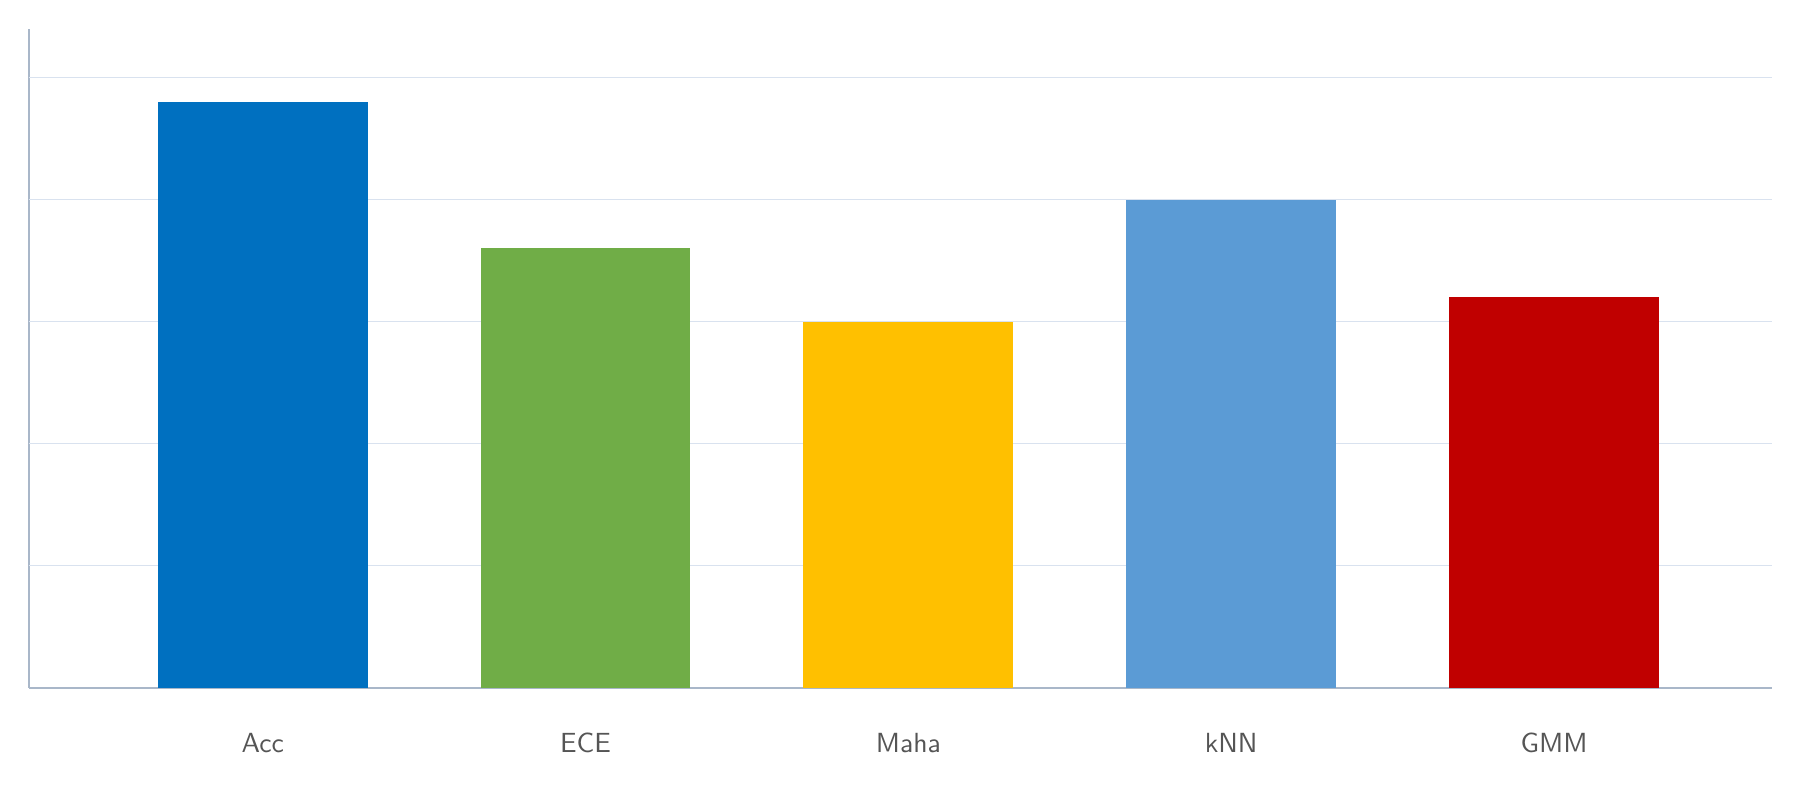
\begin{tikzpicture}[x=2.05cm,y=1.55cm]
        \draw[WantedLineStrong, line width=0.7pt] (0,0) -- (10.8,0);
        \draw[WantedLineStrong, line width=0.7pt] (0,0) -- (0,5.4);
        \foreach \y in {1,2,3,4,5} {
          \draw[WantedLine, line width=0.35pt] (0,\y) -- (10.8,\y);
        }
        \fill[WantedStatBlue] (0.8,0) rectangle (2.1,4.8);
        \fill[WantedStatGreen] (2.8,0) rectangle (4.1,3.6);
        \fill[WantedStatAmber] (4.8,0) rectangle (6.1,3.0);
        \fill[WantedStatPurple] (6.8,0) rectangle (8.1,4.0);
        \fill[WantedStatRed] (8.8,0) rectangle (10.1,3.2);
        \node[WantedMuted, font=\fontsize{10pt}{12pt}\selectfont] at (1.45,-0.45) {Acc};
        \node[WantedMuted, font=\fontsize{10pt}{12pt}\selectfont] at (3.45,-0.45) {ECE};
        \node[WantedMuted, font=\fontsize{10pt}{12pt}\selectfont] at (5.45,-0.45) {Maha};
        \node[WantedMuted, font=\fontsize{10pt}{12pt}\selectfont] at (7.45,-0.45) {kNN};
        \node[WantedMuted, font=\fontsize{10pt}{12pt}\selectfont] at (9.45,-0.45) {GMM};
      \end{tikzpicture}
    \end{center}
    \vfill
    \WantedCaption{#3}
  \end{tcolorbox}
  \vspace{10mm}
}

\newcommand{\WantedReliabilityFigure}[2]{%
  \begin{tcolorbox}[
    enhanced,
    width=\linewidth,
    height=#1,
    colback=WantedSurface,
    colframe=WantedLineStrong,
    boxrule=0.55pt,
    arc=0pt,
    left=6mm,
    right=6mm,
    top=5mm,
    bottom=5mm
  ]
    \WantedSubsectionTitle{Figure 1. Same accuracy, different reliability}
    \vfill
    \begin{center}
      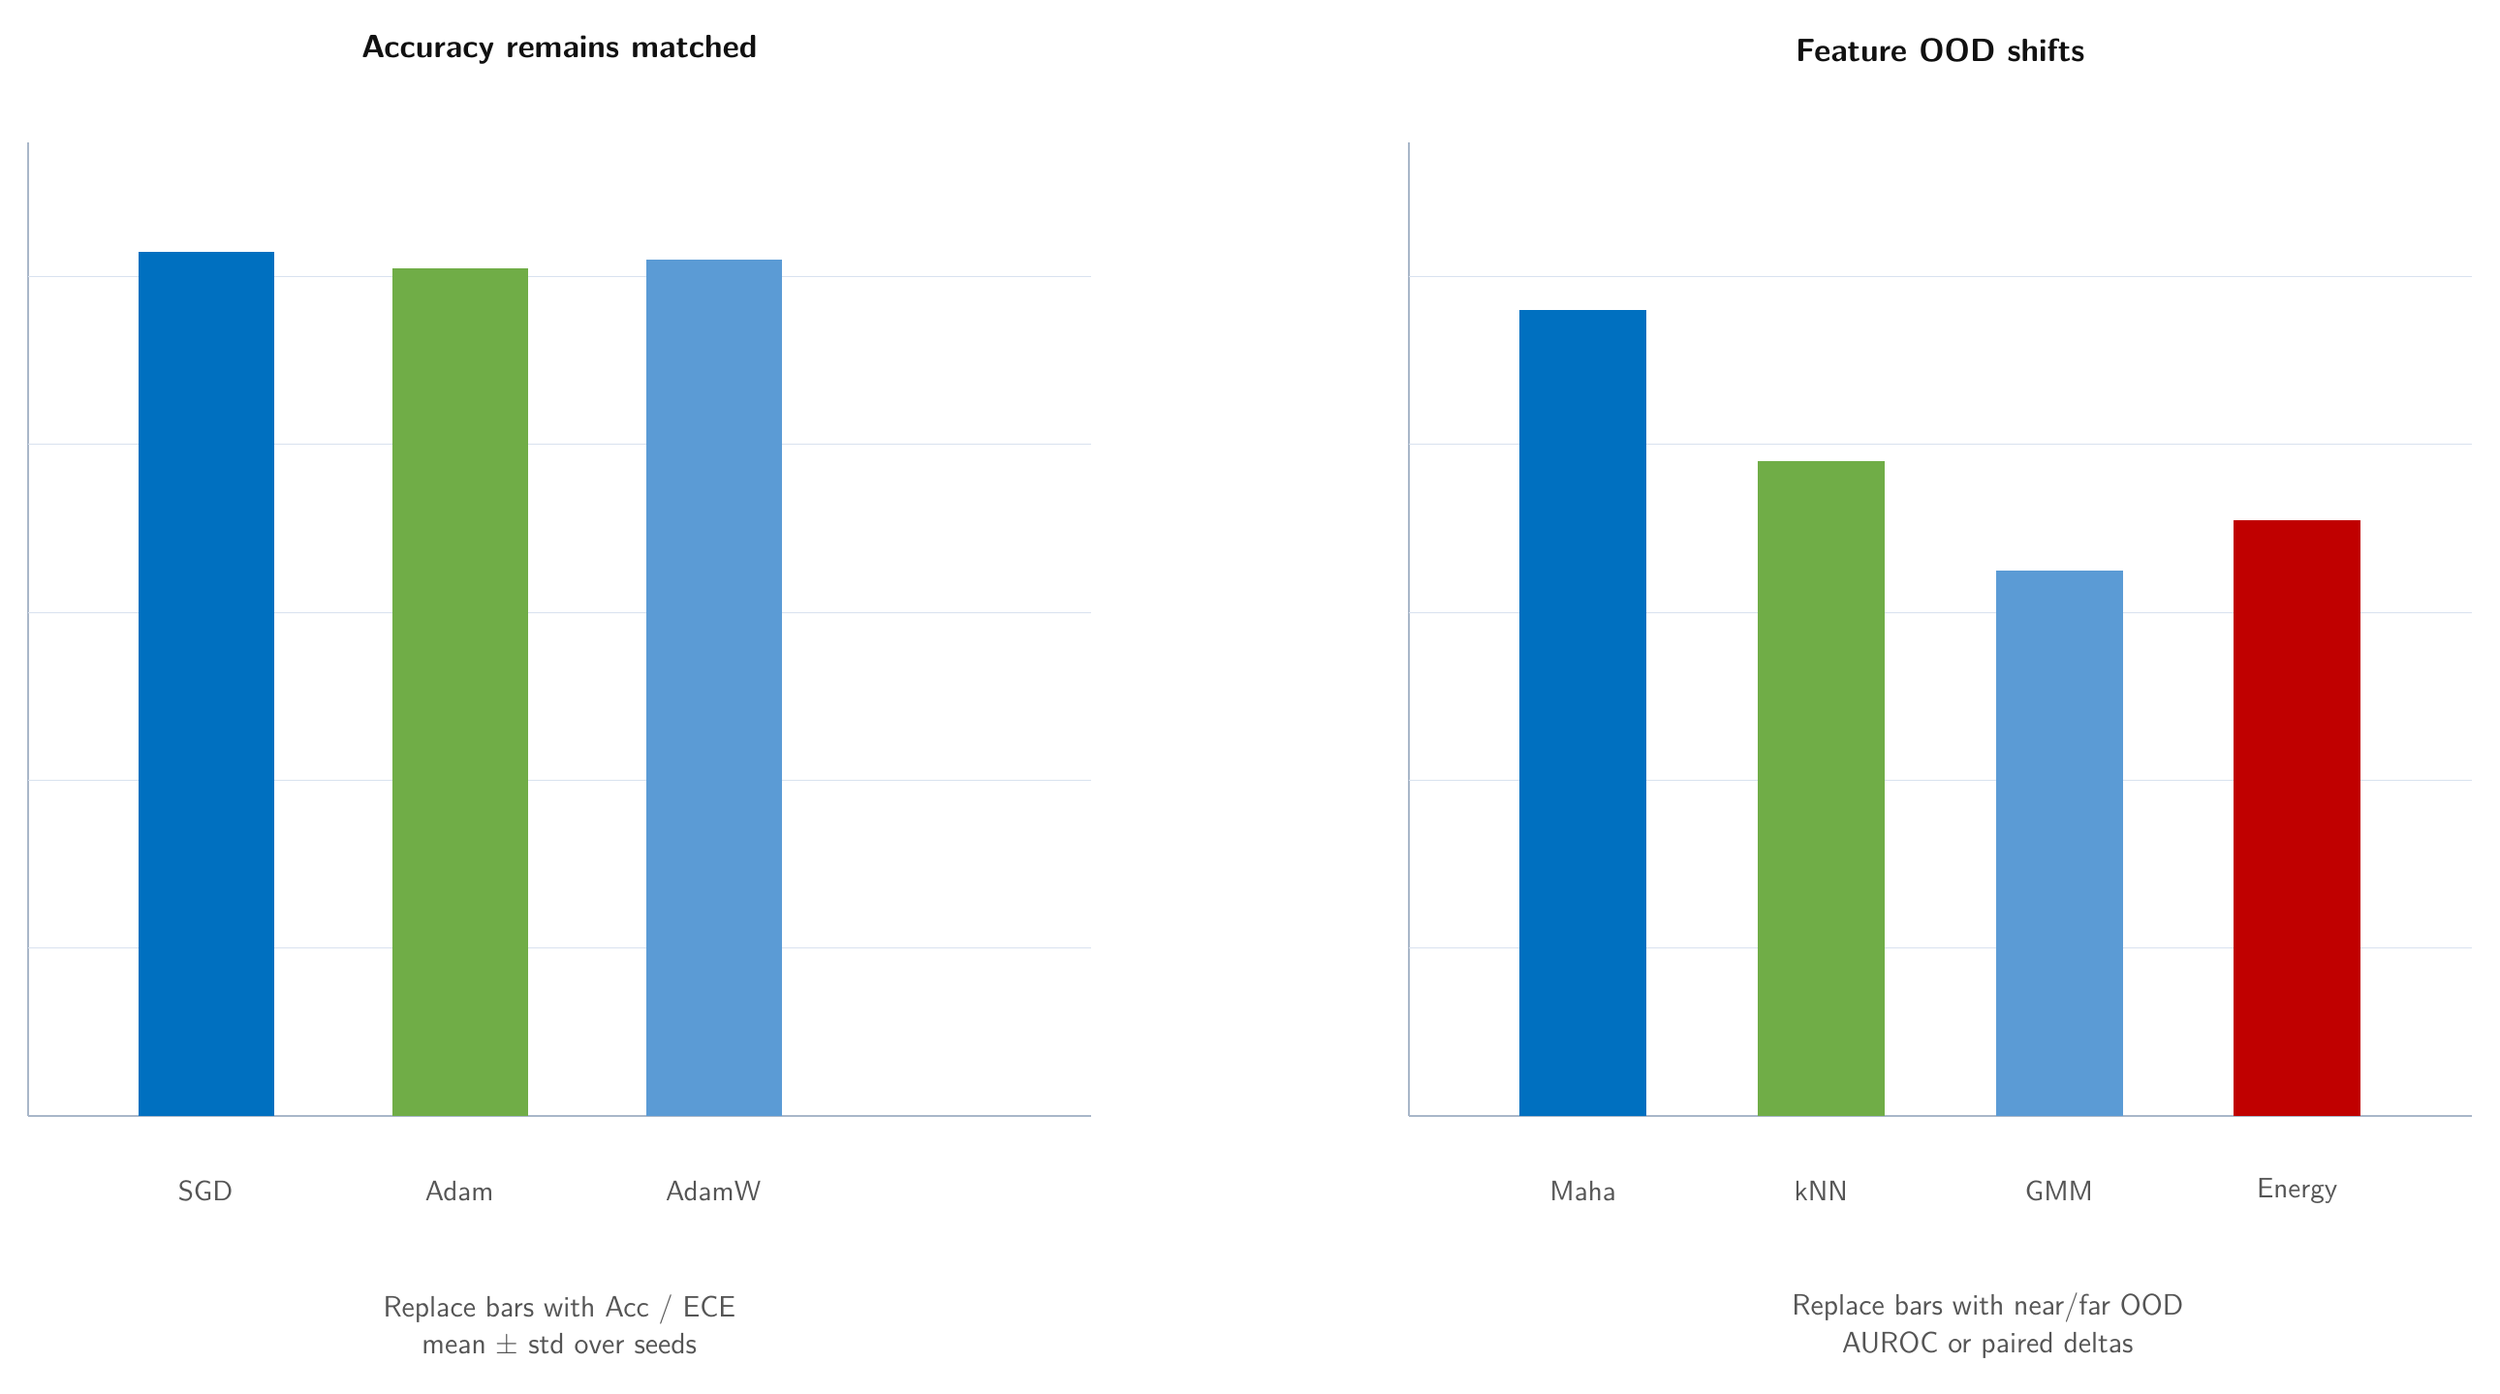
\begin{tikzpicture}[x=2.08cm,y=2.2cm]
        \foreach \x/\title in {0/{Accuracy remains matched},8.7/{Feature OOD shifts}} {
          \draw[WantedLineStrong, line width=0.7pt] (\x,0) -- ++(6.7,0);
          \draw[WantedLineStrong, line width=0.7pt] (\x,0) -- ++(0,5.8);
          \foreach \y in {1,2,3,4,5} {
            \draw[WantedLine, line width=0.35pt] (\x,\y) -- ++(6.7,0);
          }
          \node[align=center, text=WantedInk, font=\fontsize{12pt}{15pt}\selectfont\bfseries] at (\x+3.35,6.35) {\title};
        }
        \fill[WantedStatBlue] (0.7,0) rectangle (1.55,5.15);
        \fill[WantedStatGreen] (2.3,0) rectangle (3.15,5.05);
        \fill[WantedStatPurple] (3.9,0) rectangle (4.75,5.10);
        \fill[WantedStatBlue] (9.4,0) rectangle (10.2,4.80);
        \fill[WantedStatGreen] (10.9,0) rectangle (11.7,3.90);
        \fill[WantedStatPurple] (12.4,0) rectangle (13.2,3.25);
        \fill[WantedStatRed] (13.9,0) rectangle (14.7,3.55);
        \foreach \x/\label in {1.12/SGD,2.72/Adam,4.32/AdamW} {
          \node[text=WantedMuted, font=\fontsize{10.5pt}{13pt}\selectfont] at (\x,-0.45) {\label};
        }
        \foreach \x/\label in {9.8/Maha,11.3/kNN,12.8/GMM,14.3/Energy} {
          \node[text=WantedMuted, font=\fontsize{10.5pt}{13pt}\selectfont] at (\x,-0.45) {\label};
        }
        \node[align=center, text=WantedMuted, font=\fontsize{11pt}{14pt}\selectfont] at (3.35,-1.25) {Replace bars with Acc / ECE\\mean $\pm$ std over seeds};
        \node[align=center, text=WantedMuted, font=\fontsize{11pt}{14pt}\selectfont] at (12.35,-1.25) {Replace bars with near/far OOD\\AUROC or paired deltas};
      \end{tikzpicture}
    \end{center}
    \vfill
    \WantedCaption{#2}
  \end{tcolorbox}
  \vspace{10mm}
}

\newcommand{\WantedGeometryFigure}[2]{%
  \begin{tcolorbox}[
    enhanced,
    width=\linewidth,
    height=#1,
    colback=WantedSurface,
    colframe=WantedLineStrong,
    boxrule=0.55pt,
    arc=0pt,
    left=6mm,
    right=6mm,
    top=5mm,
    bottom=5mm
  ]
    \WantedSubsectionTitle{Figure 2. Feature geometry mechanism}
    \vfill
    \begin{center}
      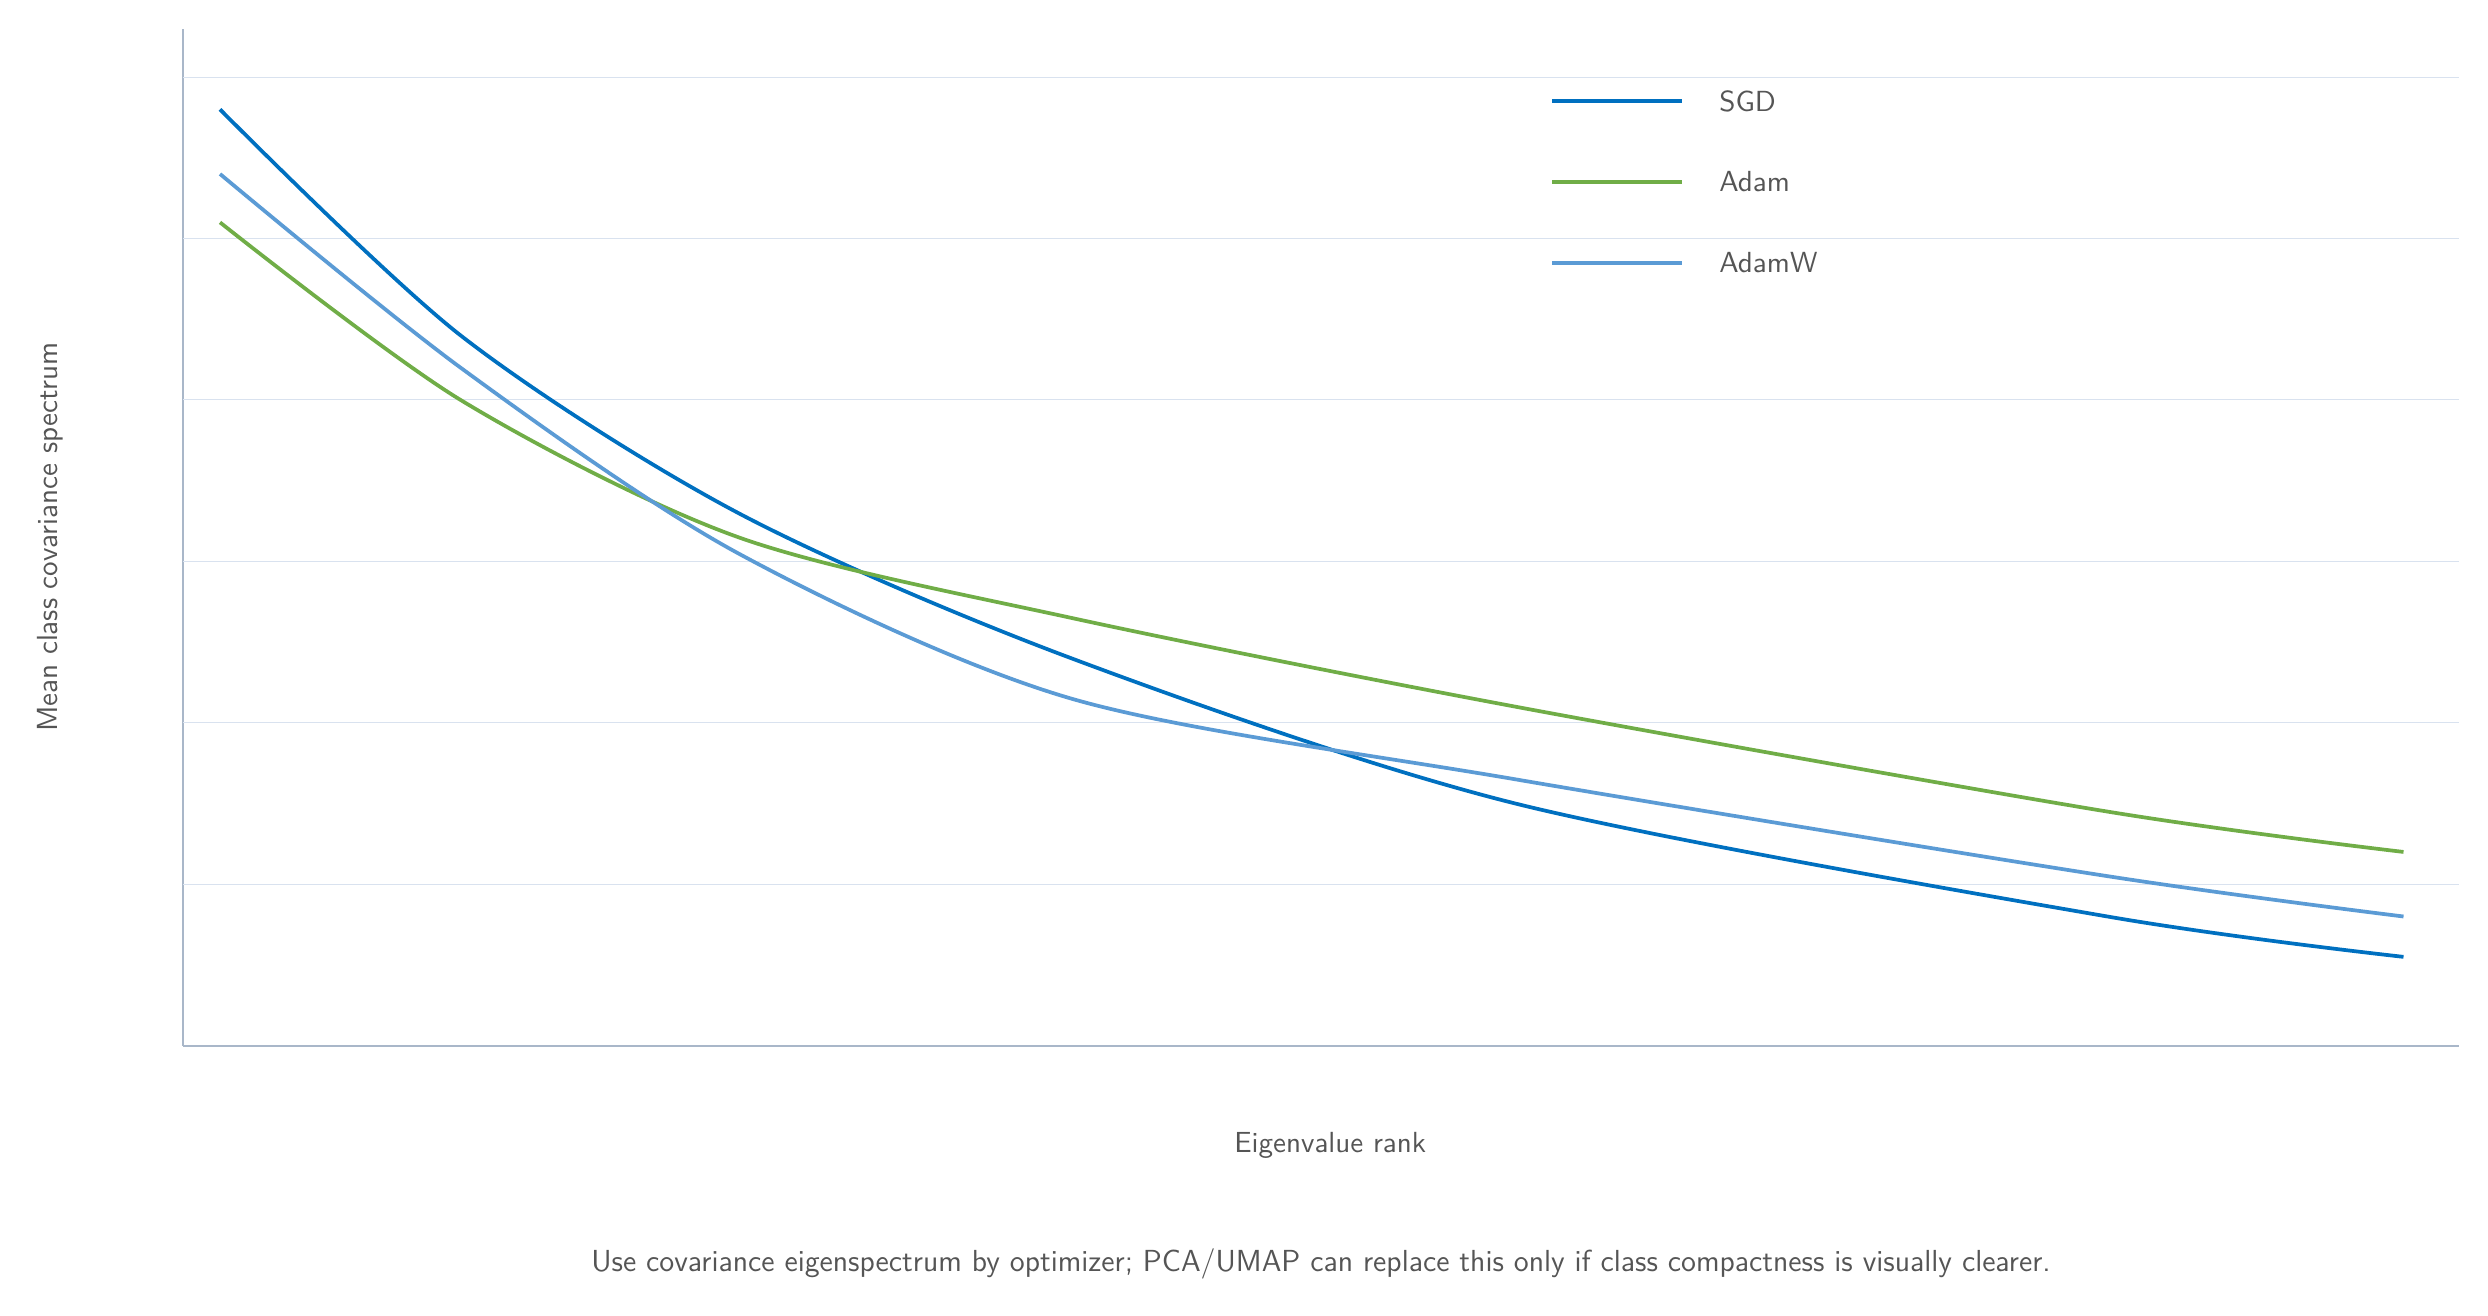
\begin{tikzpicture}[x=2.35cm,y=2.05cm]
        \draw[WantedLineStrong, line width=0.75pt] (0,0) -- (12.3,0);
        \draw[WantedLineStrong, line width=0.75pt] (0,0) -- (0,6.3);
        \foreach \y in {1,2,3,4,5,6} {
          \draw[WantedLine, line width=0.35pt] (0,\y) -- (12.3,\y);
        }
        \draw[WantedStatBlue, line width=1.35pt] plot[smooth] coordinates {(0.2,5.8) (1.5,4.4) (3.0,3.3) (4.8,2.4) (7.2,1.5) (10.4,0.8) (12.0,0.55)};
        \draw[WantedStatGreen, line width=1.35pt] plot[smooth] coordinates {(0.2,5.1) (1.5,4.0) (3.0,3.15) (4.8,2.65) (7.2,2.1) (10.4,1.45) (12.0,1.20)};
        \draw[WantedStatPurple, line width=1.35pt] plot[smooth] coordinates {(0.2,5.4) (1.5,4.2) (3.0,3.05) (4.8,2.15) (7.2,1.65) (10.4,1.05) (12.0,0.80)};
        \node[text=WantedMuted, font=\fontsize{10.5pt}{13pt}\selectfont] at (6.2,-0.62) {Eigenvalue rank};
        \node[rotate=90, text=WantedMuted, font=\fontsize{10.5pt}{13pt}\selectfont] at (-0.72,3.15) {Mean class covariance spectrum};
        \draw[WantedStatBlue, line width=1.35pt] (7.4,5.85) -- ++(0.7,0);
        \node[anchor=west, text=WantedMuted, font=\fontsize{10.5pt}{13pt}\selectfont] at (8.25,5.85) {SGD};
        \draw[WantedStatGreen, line width=1.35pt] (7.4,5.35) -- ++(0.7,0);
        \node[anchor=west, text=WantedMuted, font=\fontsize{10.5pt}{13pt}\selectfont] at (8.25,5.35) {Adam};
        \draw[WantedStatPurple, line width=1.35pt] (7.4,4.85) -- ++(0.7,0);
        \node[anchor=west, text=WantedMuted, font=\fontsize{10.5pt}{13pt}\selectfont] at (8.25,4.85) {AdamW};
        \node[align=center, text=WantedMuted, font=\fontsize{11pt}{14pt}\selectfont] at (6.15,-1.35) {Use covariance eigenspectrum by optimizer; PCA/UMAP can replace this only if class compactness is visually clearer.};
      \end{tikzpicture}
    \end{center}
    \vfill
    \WantedCaption{#2}
  \end{tcolorbox}
  \vspace{10mm}
}

\newcommand{\WantedFigureFile}[3]{%
  \begin{tcolorbox}[
    enhanced,
    width=\linewidth,
    colback=WantedSurface,
    colframe=WantedLineStrong,
    boxrule=0.55pt,
    arc=0pt,
    left=5mm,
    right=5mm,
    top=4mm,
    bottom=4mm
  ]
    \WantedSubsectionTitle{#1}
    \begin{center}
      \includegraphics[width=\linewidth]{#2}
    \end{center}
    \WantedCaption{#3}
  \end{tcolorbox}
  \vspace{8mm}
}
